% ------------ LSA-proceedings-template.tex  -- LSA proceedings template ----------------------------------------------
% created by Sarah E. Murray, 24 April 2017 based on the LSA's stylesheet
% http://journals.linguisticsociety.org/proceedings/index.php/PLSA/pages/view/instructions
%Revised by Patrick Farrell, February 1, 2019 and March 8, 2020. 
%
% ------------ begin preamble -----------------------------------------------------------------------------------------
 \documentclass[12pt,letterpaper]{article}	
% ------------ personal packages ----------------------------------------------------------------------------
\usepackage{linguex}	%http://texdoc.net/texmf-dist/doc/latex/linguex/linguex-doc.pdf
% ------------ LSA page layout and packages ----------------------------------------------------------------------------
\usepackage{times}
\usepackage{natbib}
 	\setcitestyle{semicolon,aysep={},yysep={,},notesep={; }}
\usepackage{lipsum} % this and the following package and the settings beneath them are for maintaining indentation and still having ragged-right alignment
\usepackage{ragged2e}
\setlength\RaggedRightParindent{0.3in}
\RaggedRight

\usepackage{scrextend}  % this package and the following settings are for the footnote formatting
\deffootnote[.5em]{0em}{1em}{\textsuperscript{\thefootnotemark}\,}

\newcounter{savefootnote}   % these settings allow the use of an asterisk as a footnote label (for the author line below the title.
\newcounter{symfootnote}
\newcommand{\symfootnote}[1]{%
   \setcounter{savefootnote}{\value{footnote}}%
   \setcounter{footnote}{\value{symfootnote}}%
   \ifnum\value{footnote}>8\setcounter{footnote}{0}\fi%
   \let\oldthefootnote=\thefootnote%
   \renewcommand{\thefootnote}{\fnsymbol{footnote}}%
   \footnote{#1}%
   \let\thefootnote=\oldthefootnote%
   \setcounter{symfootnote}{\value{footnote}}%
   \setcounter{footnote}{\value{savefootnote}}%
}

\usepackage[labelsep=period]{caption}

\usepackage[margin=1.0in]{geometry}
\usepackage[compact]{titlesec}
	\titleformat{\section}[runin]{\normalfont\bfseries}{\thesection.}{.5em}{}[.]
	\titleformat{\subsection}[runin]{\normalfont\scshape}{\thesubsection.}{.5em}{}[.]
	\titleformat{\subsubsection}[runin]{\normalfont\scshape}{\thesubsubsection.}{.5em}{}[.]
\usepackage[usenames,dvipsnames]{color}	
\usepackage[colorlinks,allcolors={black},urlcolor={blue}]{hyperref} 		%likes to be last package 


% -------------- personal definitions ----------------------------------------------------------------------------
\usepackage{graphicx}  
\usepackage{subcaption}
\usepackage{color}
\usepackage[export]{adjustbox}

\definecolor{Pink}{RGB}{255,50,170}
\newcommand{\jd}[1]{\textcolor{Pink}{[jd: #1]}}  
\definecolor{Blue}{RGB}{0,100,255}
\newcommand{\blue}[1]{\textcolor{Blue}{#1}}
\newcommand{\lk}[1]{\textcolor{Blue}{[lk: #1]}}

\newcommand{\citeA}{\textbf}

% -------------- LSA definitions ---------------------------------------------------------------------------------

%-------------------------------------------------------------- format abstract environment ------------------------
% Abstracts have to be 12pt, indented 1.4 inches on each side, and inline with the label
\renewenvironment{abstract}{%
\noindent\begin{minipage}{1\textwidth}
\setlength{\leftskip}{0.4in}
\setlength{\rightskip}{0.4in}
\textbf{Abstract.}}
{\end{minipage}}
%-------------------------------------------------------------- format keywords environment ----------------------
% Abstracts have to be 12pt, indented 1.4 inches on each side, and inline with the 
\newenvironment{keywords}{%
\vspace{.5em}
\noindent\begin{minipage}{1\textwidth}
\setlength{\leftskip}{0.4in}
\setlength{\rightskip}{0.4in}
\textbf{Keywords.}}
{\end{minipage}}

% ------------ end preamble -----------------------------------------------------------------------------------
% 
%
%
% ------------ begin main document ---------------------------------------------------------------------------
 
\begin{document} 

%%If using linguex, need the following commands to get correct LSA style spacing
%% these have to be after  \begin{document}
\setlength{\Extopsep}{6pt}
\setlength{\Exlabelsep}{9pt}		%effect of 0.4in indent from left text edge
%%
 
\begin{center}			%title and author lines
\normalfont\bfseries
Perceptual Difficulty Differences Predict Asymmetry in Redundant Modification with Color and Material Adjectives
\vskip .5em
\normalfont
{Leyla Kursat \& Judith Degen\symfootnote{Authors: Leyla Kursat, Stanford University (\href{mailto:lkursat@stanford.edu}{lkursat@stanford.edu}) \& Judith Degen, Stanford University (\href{mailto:jdegen@stanford.edu}{jdegen@stanford.edu})}}
% \& Judith Degen, Stanford University (\href{mailto:jdegen@stanford.edu}{jdegen@stanford.edu}).}
\vskip .5em
\end{center}

\begin{abstract}
When referring to objects, speakers are often more specific than necessary for the purpose of establishing unique reference, e.g., by producing redundant modifiers. A computational model of referring expression production that accounts for many of the key patterns in redundant adjectival modification assumes that adjectives differ in how noisy (reliable), and consequently, how useful they are for  reference. Here we investigate one hypothesis about the source of the assumed adjectival noise:  that it reflects the perceptual difficulty of establishing whether the property denoted by the adjective holds of the contextually relevant objects. 
%the prediction that systematic differences in the overmodification patterns observed for color and material adjectives can be explained by a difference in the perceptual difficulty of establishing whether objects are of a particular color or material. 
In Exp.1, we collect perceptual difficulty norms for items that vary in color and material. In Exp.~2, we test the highest (material) and lowest (color) perceptual difficulty items in a reference game and find that material is indeed less likely to be mentioned  redundantly, replicating previous work. In Exp.~3, we obtain norms for the tested items in a second perceptual difficulty measure with the aim of testing the effect of perceptual difficulty within property type. The overall results provide preliminary support for the hypothesis that the propensity to redundantly use color over material adjectives may be driven by the relative ease of assessing an object's color, compared to the relative difficulty of assessing its material.
\end{abstract}

\begin{keywords} %separated by semicolons
reference; perception; overinformativeness; redundancy; experimental pragmatics
\end{keywords}

\section{Introduction} 

Speakers often include redundant modifiers in referring expressions  (\citealt{Pechmann1989,GattEtAl2011,ArtsEtAl2011,KoolenEtAl2013}). This redundancy is typically termed \emph{overmodification} because it appears to violate the Gricean Quantity-2 maxim to say no more than necessary. However, the systematic structure in  adjectival redundancy has recently been argued to be the result of a linguistic system geared towards efficient communication (\citealt{DegenEtAl2020,RubioEtAl2019}). One way in which variability in the production of redundant referring expressions is structured is through asymmetries in the redundant use of color, size and material adjectives. When size or material is sufficient for singling out the intended referent, speakers routinely include redundant color adjectives in their utterances (e.g.,``the green plastic chair'' instead of ``the plastic chair'' in Fig.~\ref{fig:chairs}). However, in contexts where color is sufficient for unique reference, speakers rarely mention size or material redundantly (\citealt{Pechmann1989, Sedivy2003, GattEtAl2011, RubioFernandez2016, DegenEtAl2020}). Moreover, speakers' knowledge of the typicality of the properties of objects and the features of the context interact with these asymmetries. Color adjectives are more likely to be produced redundantly with increasing scene variation (\citealt{DegenEtAl2020, DaviesKatsos2013, KoolenEtAl2013}) and adjectives are more likely the be produced redundantly, the more atypical the property denoted by the adjective is for the object under discussion (\citealt{DegenEtAl2020, WesterbeekEtAl2015, Mitchell2013}).

\begin{figure}[ht]
   \centering
   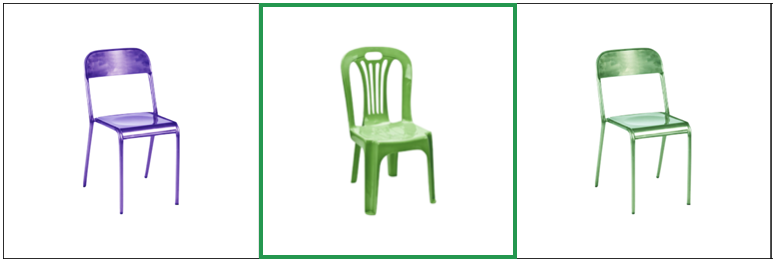
\includegraphics[width=.7\textwidth]{img/chairs.png}
   \caption{Example context where material is sufficient for unique reference. Intended referent is marked by the green border.}
   \label{fig:chairs}
\end{figure}

There are many accounts of redundancy in referring expressions, including pragmatic, semantic, lexical and visual ones. The pragmatic account proposed by \citet{Sedivy2003} builds on the contrastive effect of mentioning the color of objects that occur in predictable colors. According to this account, highly predictable properties of objects are not encoded as part of these objects' \emph{default descriptions} and therefore, their use triggers a contrastive inference and provides referential disambiguation. Although this account qualitatively captures typicality effects that have been shown to modulate redundant modification, it does not explain the source of these defaults in referential communication, nor when speakers depart from them. In addition to listeners' expectations of informativity, production of overinformative referring expressions has been shown to depend on the object category (\citealt{RubioFernandez2016}) and the semantics of the adjective involved (\citealt{RubioEtAl2019, Sedivy2003}). Relatedly, based on a comparison of eye movement patterns in the online comprehension of color and scalar adjectives, \citet{AparicioEtAl2018} report that processing  differences may be the attributable to differences in the semantics of the adjectives, i.e., the result of differences in processing relative vs.~absolute adjectives. However, explanations of adjectival production asymmetries that rest on differences in the semantics of the adjectives do not capture the fine-grained context-dependence of redundant modification. For instance, \citet{ViethenEtAl2017} showed that  a decrease in color contrast between displayed objects reduces the use of color adjectives in referring expressions. Accounts that focus on the role of perceptual factors in redundant modification take into consideration such contextual effects and argue that redundant adjective use is sensitive to the relative visual salience of properties  adjectives denote (\citealt{Taranskeen2015, RubioEtAl2019, EttingerFernandez2020}), such that speakers choose utterances with considerations of their perceptual utility for the listener. That is, speakers are not only aiming to be informative but rather efficient in their utterance choices, in order to facilitate the listener's target search. 

In this paper, we explore a hypothesis aligned with accounts of the production of referring expression that center the communicative efficiency of perceptually salient properties of objects (\citealt{EttingerFernandez2020}), motivated by a recent computational model of referring expression production that spells out why redundant referring expressions may be more communicatively efficient than their non-redundant counterparts (\citealt{DegenEtAl2020}). Couched within the Rational Speech Act (RSA) framework (\citealt{Goodman2016}), this model treats speakers and listeners as agents recursively reasoning about each other's mental states to communicate. The simple RSA model assumes that objects have deterministic lexical meanings and that speakers choose utterances that maximize informativeness with respect to those meanings. This model doesn't generate overinformative referring expressions mainly because it calculates the informativeness (and cost) of mentioning the redundant property to be equal to the informativeness of mentioning the alternative (only mentioning the sufficient property). \citet{DegenEtAl2020} extend this model by focusing on the calculation of informativeness and relaxing the Boolean semantics to a non-deterministic continuous semantics that returns real values between 0 and 1. By allowing utterances to be informative about objects to varying degrees, this continuous semantics assumes that adjectives differ in how noisy or unreliable, and consequently, how useful they are for the purpose of establishing reference. The noisier the adjective, the less useful it is for allowing a listener to infer the intended referent. In contrast, the more reliable the adjective, the more useful it is even when used redundantly, because it allows for restricting the domain of reference more faithfully than the noisier adjectives do. \citet{DegenEtAl2020} show that assuming size adjectives are noisier than color adjectives accounts for asymmetries in the redundant production of color vs.~size adjectives, and effects of scene complexity on redundant modification fall out of the model for free. However, this account raises the crucial question regarding the source of the presumed adjectival noise. The authors speculatively raise a few possibilities for what the noise might reflect. For instance, it could represent the perceptual difficulty of establishing whether an object exhibits the property denoted by the adjective. Alternatively, it might reflect the past communicative success in using a particular adjective type. It may also reflect the agent's prior beliefs about the correlations between features of objects. 

Here, we take the first step in testing the first possibility, which we spell out in the \emph{Perceptual Difficulty Hypothesis}: that the noise term reflects the perceptual difficulty of establishing whether the property denoted by the adjective holds of the contextually relevant objects in the domain of color and material adjectives. The prediction is that systematic differences in the redundant modification patterns observed for color and material adjectives can be explained by a difference in perceptual difficulty of establishing whether objects are of a particular color or material. The more difficult it is to judge whether an object has a property, the less likely speakers should be to redundantly mention that property. In Exp.1, we norm the perceptual difficulty associated with establishing whether an object exhibits a color or material and select the highest and lowest perceptual difficulty objects  for testing in Exp.~2. In Exp.~2, we test in an interactive reference game whether adjectives that denote more perceptually difficult property---material---are indeed less frequently produced redundantly than the perceptually easier to establish color. Finally, in Exp.~3, we replicate the perceptual difficulty measures from Exp.~1 and investigate the role of perceptual difficulty within property type.

%We investigate the role of perceptual difficulty in the production of overinformative referring expressions. We show that perceptual difficulty associated with establishing whether an object exhibits a property could be a contributing factor to the noise term assumed by the computational model of referring expression production developed by \citet{DegenEtAl2020}. In doing so, we provide a pragmatic explanation for how systematically related perceptual factors are to informativity calculations.

\section{Experiment 1: Measuring perceptual difficulty} 

First, we collected perceptual difficulty norms for assessing the color and material  of 81 images. Through a timed forced choice task we measured the out-of-context perceptual difficulty of establishing whether  objects have a particular color or are made of a particular material.

\subsection{Participants} 

We recruited 120 participants through Amazon Mechanical Turk. We excluded participants who were self-reported non-native English speakers (n=4) and participants with accuracy lower than 75\% (n=11).

\subsection{Procedure} 

Participants saw images of objects alongside a color or material adjective and were asked to indicate whether the object had the property denoted by the adjective or not. Their task was to indicate ``yes" or ``no" by pressing the F or J key as quickly as possible. If participants did not respond within 4 seconds, the trial timed out. When participants responded correctly, a green border appeared around their selection, and when they responded incorrectly a red border appeared.

We collected perceptual difficulty norms for 12 objects that each occurred in two or three different materials and in three different colors. All resulting 81 images were separately normed for object nameability, property nameability, object typicality and property typicality. Every participant saw each image once and we collected 30 judgements for each image with matching and non-matching color and material adjectives. Color and material adjectives that didn't match the images were randomly selected for each participant from a pool of adjectives denoting properties of other images in the experiment.

\subsection{Results} 

Figure~\ref{fig:exp1} shows the proportion and response times of correct responses to color and material adjectives.  In order to assess whether material is more perceptually difficult to assess than color, we conducted two types of analyses. First, we analyzed the responses by conducting a mixed effects logistic regression predicting the log odds of making an error from a dummy-coded fixed effect of property type (reference level: `color'). Second, we analyzed the response times of correct responses by conducting a mixed effects linear regression predicting log-transformed response time from property type. Both models included the maximal random effects structure justified by the design: by-item and by-participant intercepts and by-participant slopes for property type. Overall, material adjectives resulted in higher error rates ($\beta$= 0.48, $SE$=0.12, $p$$<$.0001) and greater response times ($\beta$=5.44, $SE$=4.74, t=11.49, $p$$<$.0001) than color adjectives, suggesting that material is indeed a more perceptually difficult property to establish than color.  These results provide preliminary evidence for the Perceptual Difficulty Hypothesis. 

\begin{figure}[ht]
\centering
\begin{subfigure}{.4\textwidth}
\centering
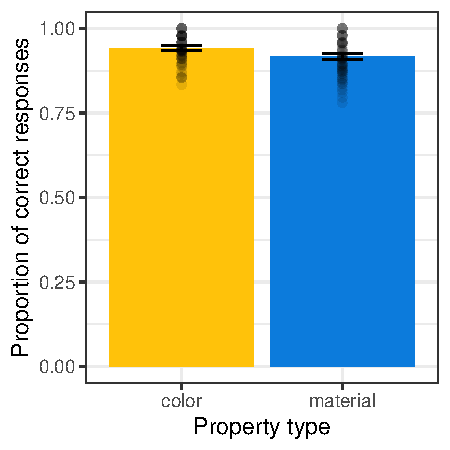
\includegraphics[width=\textwidth]{plots/exp1_proportion.pdf}
\caption{Proportion of correct responses.}
\label{fig:exp1_a}
\end{subfigure} \hspace{9mm}
\begin{subfigure}{.4 \textwidth}
\centering
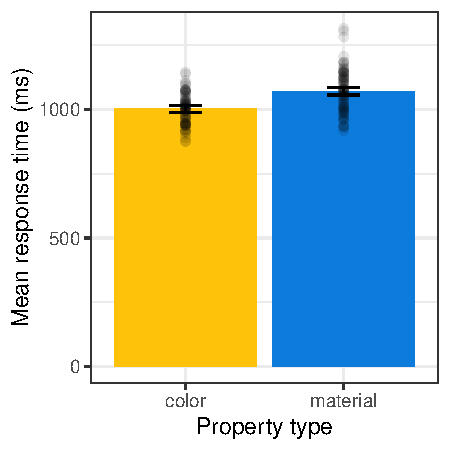
\includegraphics[width=\textwidth]{plots/exp1_rt.pdf}
\caption{Response times for correct responses.}
\label{fig:exp1_b}
\end{subfigure}
\caption{Responses to color and material adjectives in Experiment 1. Individual dots represent participant means and error bars indicate 95\% bootstrapped confidence intervals.}
\label{fig:exp1}
\end{figure}  

In order to determine a set of items to use for the production study in Exp.~2, we selected two sets of items from the total set of normed items: a \textit{high difficulty} set of perceptually difficult image-adjective pairs and a  \textit{low difficulty} set of perceptually less difficult image-adjective pairs. To create these sets, we first ordered the image-word combinations along six different measures: (1) response time regardless of response correctness (correct, incorrect) and regardless of  response type (yes, no), (2) response time for only correct responses, regardless of response type, (3) response time for only correct `yes' responses, (4) response time for only correct `no' responses, (5) error rate regardless of response type, (6) error rate  only among `yes' responses (7) error rate  only among `no' responses. Image-material adjective pairs were consistently among the highest difficulty items and image-color adjective pairs were consistently among the lowest difficulty items. We thus selected the 8  image-material adjective pairs with the consistently highest error rate and response times for the \textit{high difficulty} set, and the 8 image-color adjective pairs with the consistently lowest error rate and response times for the \textit{low difficulty} set. We used these final 16 items as target items in Exp.~2. 

\section{Experiment 2: Production of referring expressions} 

The goal of Exp.~2 was to measure the production probability of redundant color and material adjectives for the items normed in Exp.~1. In a free production interactive reference game we tested whether the less perceptually difficult color was more frequently produced redundantly than the more perceptually difficult material.\footnote{This  experiment was preregistered at \href{https://osf.io/57c6u}{https://osf.io/57c6u}. Experimental materials, data, and analysis files for all three experiments can be accessed at \href{https://github.com/leylakursat/perceptual_difficulty}{https://github.com/leylakursat/perceptual\_difficulty}.}

\subsection{Participants} 

We recruited 100 participants through Amazon Mechanical Turk and randomly paired them into speaker-listener dyads to play a real time communication game (50 pairs, \citealt{Hawkins2015}). We excluded games where participants reported a native language different from English (n=5).

\begin{figure}[h]
   \centering
   \begin{minipage}[t]{0.48\linewidth}
   \centering
   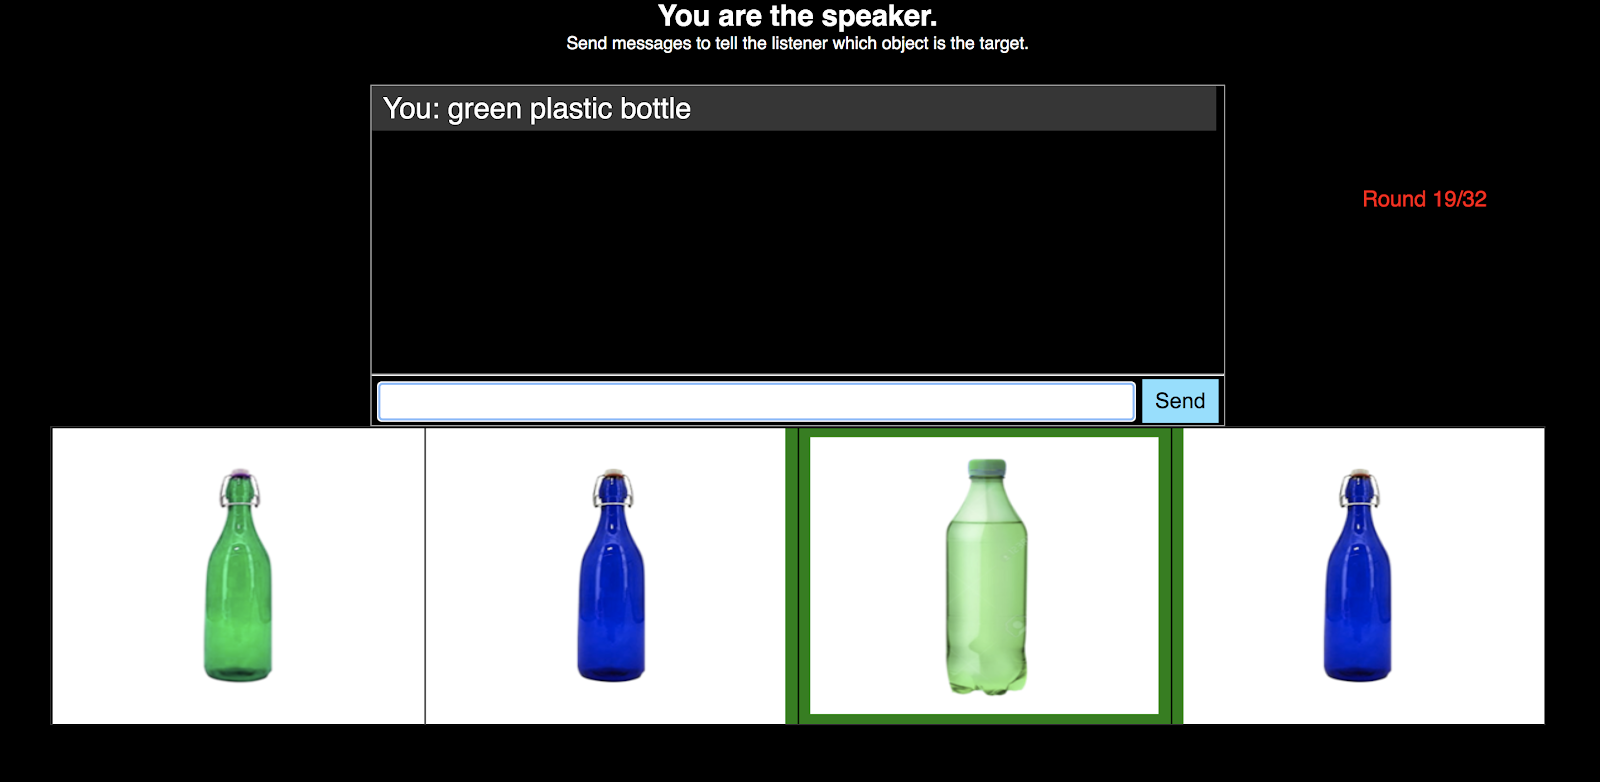
\includegraphics[width=\textwidth, frame]{img/exp2_trial.png}
   \captionof{figure}{Example display from Exp.~2: speaker's perspective on a \textit{low-difficulty (color redundant)} trial.}
   \label{fig:exp2_trial}
   \end{minipage}\hfill%
   \begin{minipage}[t]{0.48\linewidth}
   \centering
   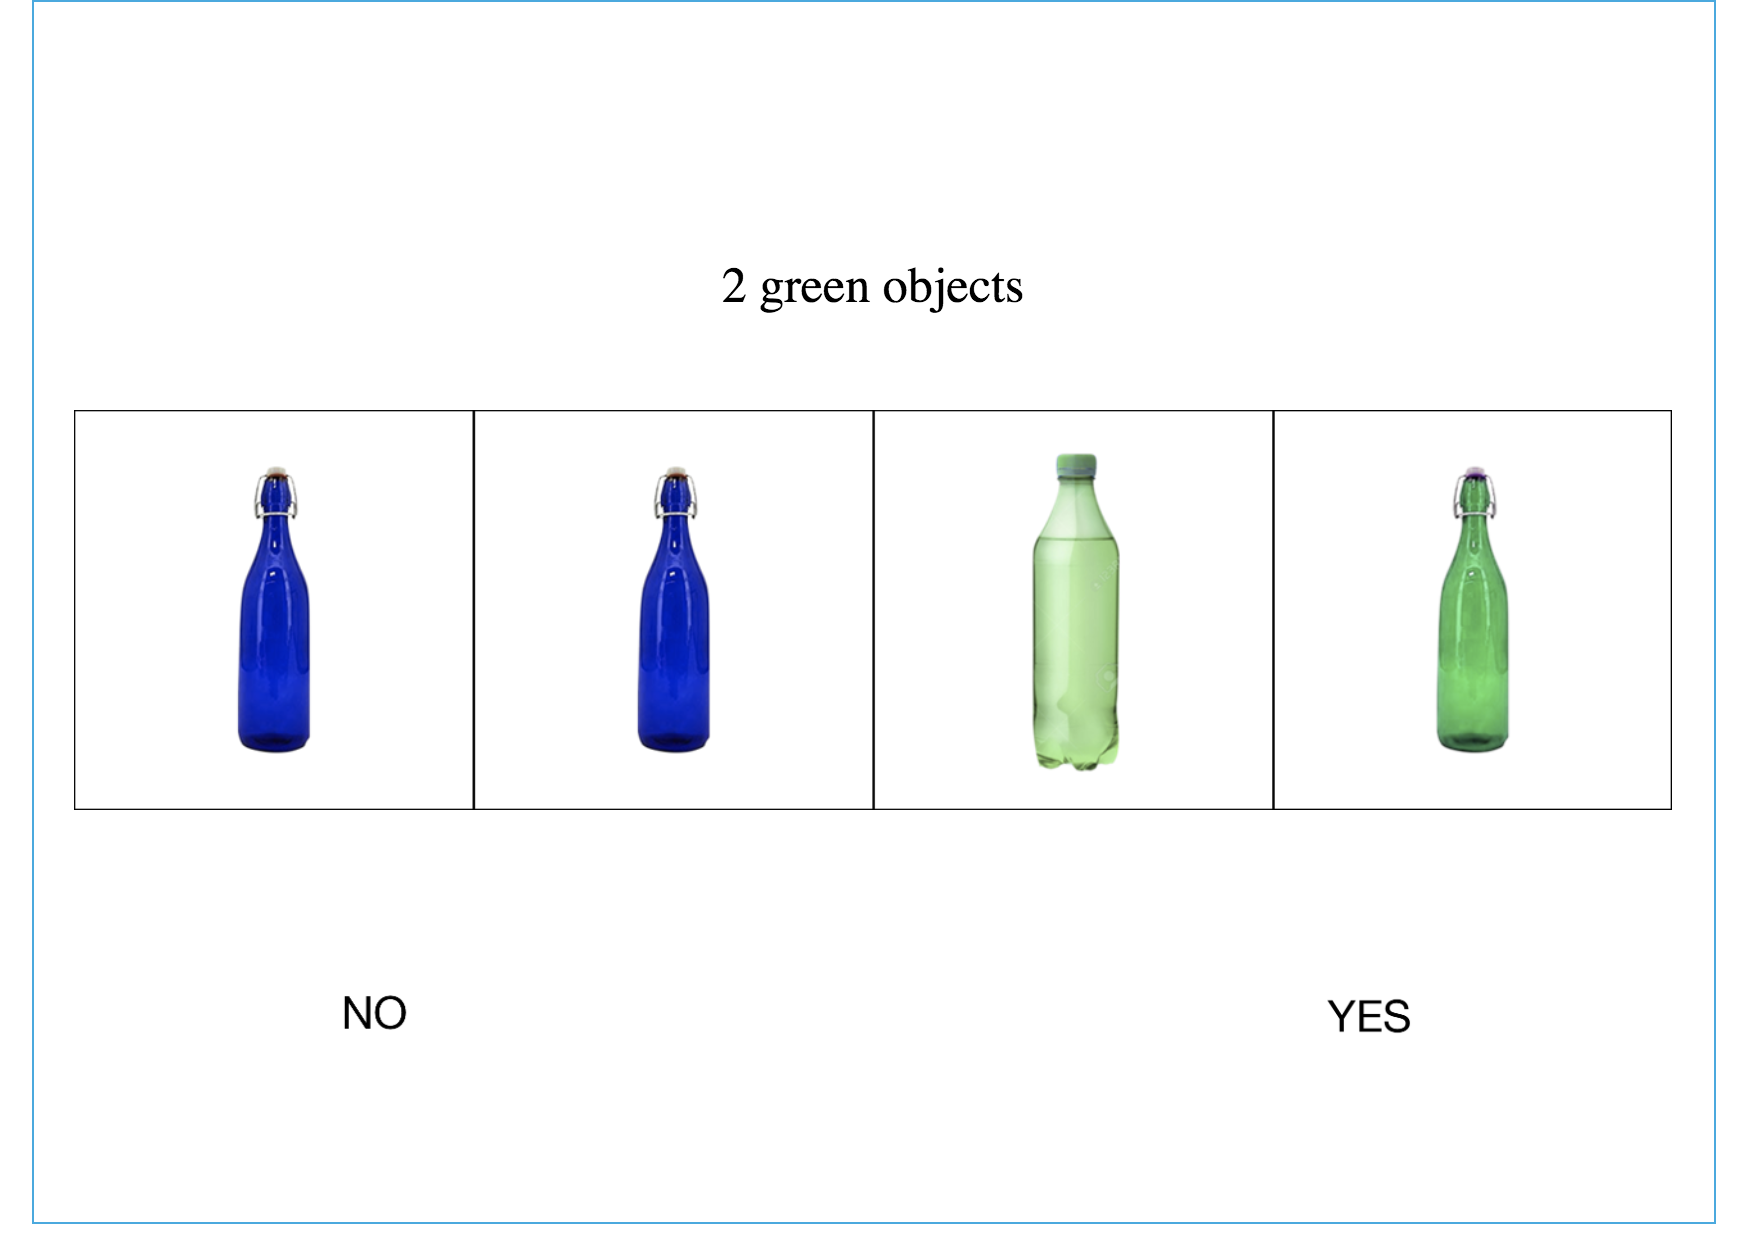
\includegraphics[width=\textwidth, frame]{img/exp3_trial.png}
   \captionof{figure}{Example display from Exp.~3: color trial with correct number.}
   \label{fig:exp3_trial}
   \end{minipage}
\end{figure}


\subsection{Procedure} 

On each trial, participants saw a display with 4 images and chat box. Both the speaker and the listener saw the same images in different positions. One of the images was designated as the target image, and marked by a green border in the speaker's display. The speaker's task was to describe this target image to the listener using the chat box to send messages. The listener's task was to guess the target image by clicking. After the listener made a selection, both participants received feedback about whether the target image was selected and advanced to the next trial. 

Participants completed 32 trials. Of these, half were critical trials and half were filler trials. On critical trials (Figure~\ref{fig:exp2_trial}), the 4 images were of the same object type (e.g., 4 bottles) and either \textit{color} or \textit{material} was redundant for distinguishing the target. One of the images, the competitor, always shared the redundant property with the target and the two distractors shared the sufficient property with the competitor.\footnote{This was one of the conditions identified by \citet{DegenEtAl2020} as resulting in a high probability of redundant modification.} On 8 \emph{high-difficulty / material redundant} trials, mentioning the material was redundant; on 8 \emph{low-difficulty / color redundant} trials, color was redundant. On filler trials, the 4 images contained different objects and both color and material were redundant. Filler items were of 4 different types: the competitor either shared the color, material, both or none of the properties with the target. 

\begin{figure}[hb]
\centering
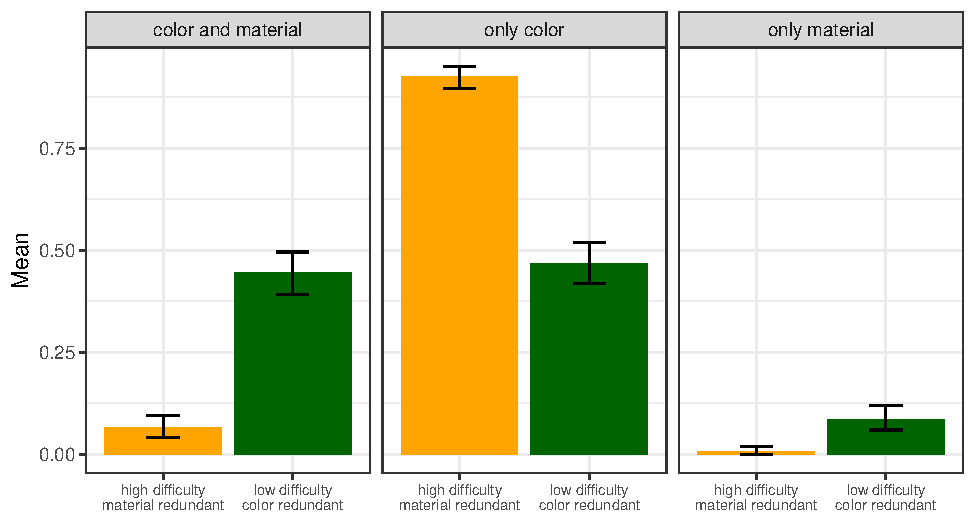
\includegraphics[width=.8\textwidth]{plots/exp2_proportion.pdf}
\caption{Proportion of redundant ``color and material" utterances vs.~non-redundant utterances on high and low difficulty trials. Error bars indicate 95\% bootstrapped confidence intervals}
\label{fig:exp2_proportion}
\end{figure}

\subsection{Results and discussion}

To investigate the use of redundant adjectives, we first classified the produced utterances as redundant ``color and material"  (e.g., \textit{the blue metal chair}), minimal or underinformative ``only color" (e.g., \textit{the green cup}) and minimal or underinformative ``only material" (e.g., \textit{the metal chair}). Proportion of redundant  and non-redundant referring expressions are shown in Figure~\ref{fig:exp2_proportion}. 

To assess whether color was more likely to be mentioned redundantly than material, we conducted a mixed effects logistic regression predicting redundant adjective use from a dummy-coded fixed effect of redundant property  (reference level: `color'), with random by-subject and by-item intercepts and slopes for redundant property. There was a main effect of redundant property, such that speakers were more likely to redundantly mention color than material ($\beta$= 2.32, $SE$=0.64, $p$$<$.0001), replicating the previously observed asymmetry between redundant modification with color and material adjectives on a new set of items (\citealt{Sedivy2005,EttingerFernandez2020}). Our analysis of the responses to filler trials showed that the preference to mention color transferred to trials in which neither color nor material mention was required for unique reference.

\begin{figure}[ht]
   \centering
   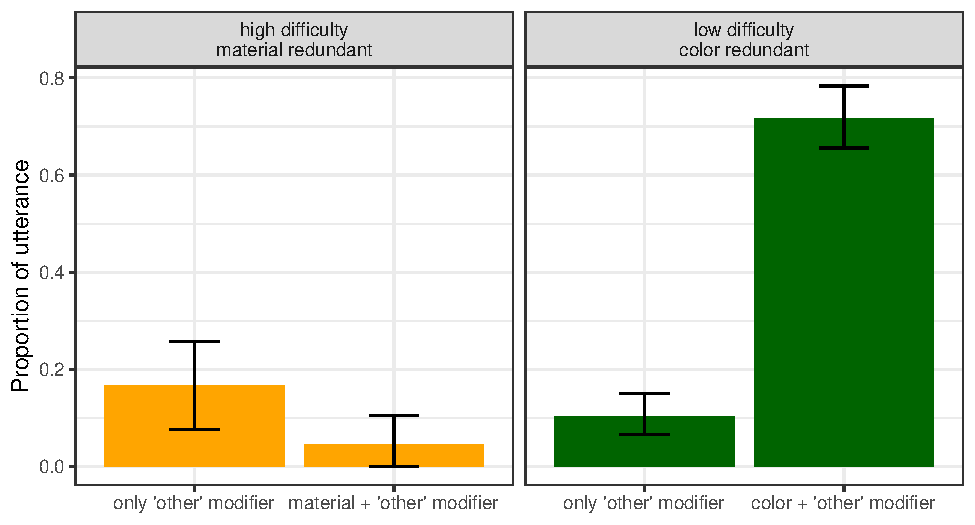
\includegraphics[width=.8\textwidth]{plots/exp2_other.pdf}
   \caption{Proportion of utterance of `other" modifier types with modifier denoting the redundant property. Error bars indicate 95\% bootstrapped confidence intervals} 
   \label{fig:exp2_other}
   \end{figure}

What is not visible in Figure~\ref{fig:exp2_proportion} is that on 39\% of trials, participants mentioned  modifiers other than the expected color and material adjectives to refer to the target. These modifiers included shape (\textit{rectangular table, square table}), size (\textit{long table, short boot}), shade (\textit{dark blue plate, light green vase}) and other (\textit{solo cup, shiny pitcher}) modifiers. To assess whether the use of other modifiers contains any additional evidence for an asymmetry in preference for using color versus material adjectives, Figure~\ref{fig:exp2_other} shows the distribution of ``other" modifiers produced instead of the sufficient adjective, i.e., the proportion of trials on which speakers preferred to avoid mentioning the sufficient property altogether. While the rate of other modifier uses was generally low, an exception is the color redundant condition, where material would have been sufficient for identifying the referent: in this case, participants frequently avoided producing the material modifier by instead mentioning color together with another property that correlated with the material, e.g., \emph{shiny blue table} instead of \emph{metal table}, or by modifying color directly, e.g., \emph{dark blue plate}. These results provide further evidence that participants dispreferred mentioning material.

% The full data pattern with color, material and other modifiers revealed that when material was the redundant feature, participants mentioned only the color, and when color was the redundant feature, they either produced color-and-material utterances or overmodified with color and used a modifier denoting a property other than color or material. 

Together with the norms from Exp.~1, these results suggest that the more difficult it is to judge whether an object has a property, the less likely speakers are to redundantly mention that property, providing further  support for the Perceptual Difficulty Hypothesis. However, a stronger test of the hypothesis would be to ask whether within-property differences in perceptual difficulty are predictive of within-adjective-type variability in redundant modification; e.g., whether an easier-to-perceive material is mentioned redundantly more frequently than a harder-to-perceive material. Unfortunately, the within-property differences in perceptual difficulty for the tested items were very small on both the error measure and the response time measure elicited in Exp.~1. Moreover, the items in this study were specifically selected for maximal perceptual difficulty differences between color and material. The combination of the very low amount of variability in perceptual difficulty within property and the relatively stark separation of color and material in perceptual difficulty space thus does not afford us the power to test the stronger version of the Perceptual Difficulty Hypothesis with the data we have reported thus far. Exp.~3 aims to remedy part of this problem by obtaining perceptual difficulty estimates for the same items with a more sensitive perceptual difficulty measure that is likely to yield greater within-property variability.

\section{Experiment 3: Perceptual difficulty in context} 

The goal of Exp.~3 was to obtain an additional measure of perceptual difficulty for the items used in Exp.~2, both to replicate the results of Exp.~1 on a second measure and to subject the Perceptual Difficulty Hypothesis to a stronger test by probing within-property perceptual difficulty effects on redundant adjective use measured in Exp.~2.

\subsection{Participants} 

We recruited 400 participants through Prolific. We excluded participants with accuracy lower than 75\% (n=24) and responses that were 2.5 standard deviations away from the mean response time (2\% of all trials).
\subsection{Procedure} 

Exp.~3 was identical to Exp.~1 but instead of seeing the images in isolation, participants saw the displays from the production experiment (Exp.~2). These displays appeared with short descriptions that were of the form ``X [adjective] objects" and included a number and either a color or material adjective (see Figure~\ref{fig:exp3_trial}). Participants were asked to press a button as quickly as possible to indicate whether the display contained the described objects or not. For example, in Fig.~\ref{fig:exp3_trial}, ``2 green objects" was true but ``2 plastic objects" was false. On half of the trials, the statement was correct and on the other half, it was incorrect. The use of color and material adjectives was also balanced. We collected 100 judgements for each property in the display, for all the different displays. Each participant completed 31 trials.

\subsection{Results} 

Figure~\ref{fig:exp3} shows the proportion and response times of correct responses to color and material adjectives.  We first report analyses to assess whether the results of Exp.~1 replicate on this perceptual difficulty task. We then report analyses aimed at testing the strong version of the Perceptual Difficulty Hypothesis.

As in Exp.~1, in order to assess whether material is more perceptually difficult to assess than color, we conducted two types of analyses. First, we analyzed the responses by conducting a mixed effects logistic regression predicting the log odds of making an error from a dummy-coded fixed effect of property type (reference level: `color'). Second, we analyzed the response times of correct responses by conducting a mixed effects linear regression predicting log-tranformed response time from property type  (reference level: `color'). Both models included the maximal random effects structure justified by the design: by-item and by-participant intercepts and by-participant slopes for property type. Overall, material adjectives resulted in higher error rates ($\beta$= 0.96, $SE$=0.09, $p$$<$.0001) and greater response times ($\beta$=0.24, $SE$=0.018, t=-59.62, $p$$<$.0001) than color adjectives, replicating the results of Exp.~1. 

\begin{figure}[ht]
   \centering
   \begin{subfigure}{.4\textwidth}
   \centering
   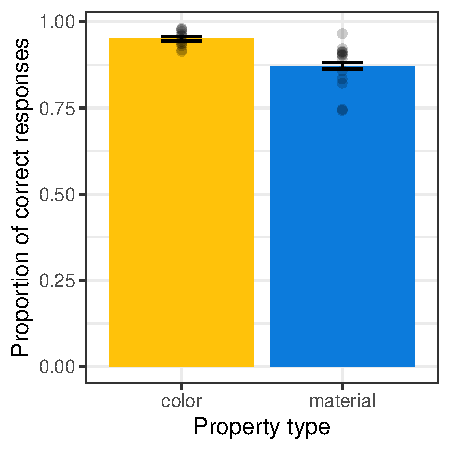
\includegraphics[width=\textwidth]{plots/exp3_proportion.pdf}
   \caption{Proportion of correct responses.}
   \label{fig:exp3_a}
   \end{subfigure} \hspace{9mm}
   \begin{subfigure}{.4 \textwidth}
   \centering
   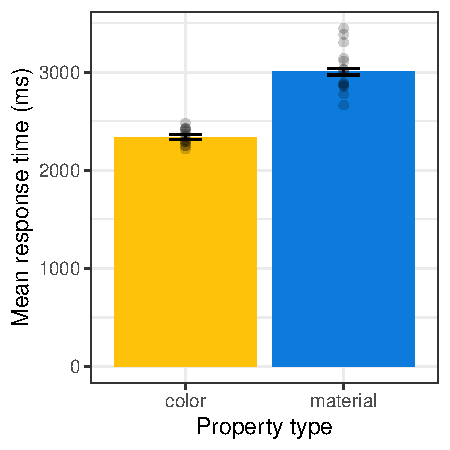
\includegraphics[width=\textwidth]{plots/exp3_rt.pdf}
   \caption{Response times for correct responses.}
   \label{fig:exp3_b}
   \end{subfigure}
   \caption{Responses to color and material adjectives in Experiment 3. Individual dots represent participant means and error bars indicate 95\% bootstrapped confidence intervals}
   \label{fig:exp3}
\end{figure}   

To address the strong version of the Perceptual Difficulty Hypothesis, namely that perceptual difficulty modulates redundancy above and byeond property type, an additional analysis step was necessary. Because property type is a strong predictor of response time and property type and response time would be highly collinear in a regression analysis, we first regressed log-transformed response times against property type using a simple linear model. % predicting log-transformed response time from trial type ($\beta$= -0.26, $SE$=0.004, t=-71.24, $p$$<$.0001).  we first analyzed the absolute response times to redundant and sufficient properties of target items of Exp.~2. In order to identify the individual contribution of trial type and mean response time (to redundant adjective) on redundant adjective use, we first performed a residualization step. Since 
We then used the residuals of this model as the predictor in a mixed effects logistic regression predicting redundant adjective use in Exp.~2 from the mean-centered predictors  property type, perceptual difficulty (i.e., residualized response time), and their interaction. We replicated the effect of property type on response time ($\beta$= 7.43, $SE$=2.27, $p$$<$.001) but found neither a main effect of perceptual difficulty ($\beta$= -11.3, $SE$=16.41, $p$$=$.49) nor an interaction between property type and perceptual difficulty ($\beta$= 13.57, $SE$=31.87, $p$$=$.67) on redundant adjective use. This analysis suggests that there is no evidence for within-property effects of perceptual difficulty on redundant adjective use.

To further test the strong version of the Perceptual Difficulty Hypothesis, we used another measure of perceptual difficulty: the relative perceptual difficulty of assessing the sufficient property compared to the redundant property. We computed the log ratio of mean sufficient property response time to   mean redundant property response time and performed the same residualization step described above. Again, there was no significant effect of perceptual difficulty above and beyond property type ($\beta$=5.31, $SE$=3.87, $p$$=$.17)).


\section{General discussion} 

We tested the role of perceptual difficulty in explaining the asymmetry in redundant color and material adjective use in referring expressions. The prediction generated by the Perceptual Difficulty Hypothesis is that the more difficult it to establish whether an object is of a particular color or material, the less likely speakers should be to redundantly mention that property.

There are two versions of the Perceptual Difficulty Hypothesis. The work thus far provides evidence for the weak version of this hypothesis, that the propensity to redundantly use color and material adjectives may be driven by the asymmetry in the perceptual difficulty involved in establishing whether or not a particular object is of a particular color or material. Exp.~1 and Exp.~3 both provide support for this hypothesis, since in both experiments color adjectives generally resulted in lower error rates and lower response times than material adjectives. Under the strong version of the hypothesis, perceptual difficulty should modulate redundancy within property type, such that, e.g., easier-to-perceive material should be mentioned redundantly more frequently than  harder-to-perceive material. The data collected thus far does not provide evidence for the strong version of the hypothesis. This may be either because the strong version does not hold, or for a simpler, methodological reason: the items we selected were structured such that between-property differences in perceptual difficulty were maximized, and within-property differences were minimized. Follow-up work should assess the strong version of the hypothesis on a separate set of items that includes perceptual difficulty overlap between color and material as well as greater within-property variability in perceptual difficulty. 

It is possible that the effects of perceptual difficulty on redundant adjectival modification are confounded by the retrieval difficulty of the adjectives, in line with availability-based production theories \jd{include ref to bock 1987 (JML) and ferreira and dell 2000 (Cognitive Psychology)}. That is, it may be that material adjectives are mentioned less frequently simply because they are harder to retrieve from memory, in turn perhaps because they are less frequent in the input. A cursory corpus search makes this possibility unlikely: in the Google Books Ngram Viewer (based on a corpus of over 20 million print books), the material noun combinations used in our experiments were less frequent than the color noun combinations, showing that retrieval formalized in terms of frequency, can't account for these results. \jd{hold on, the material noun combinations being less frequent is exactly what the availability-based production people would need to say it's just a retrieval story! didn't you show me results where the color noun combinations were less frequent???}

The results overall are consistent with efficiency-based accounts of redundant adjective use \jd{cite rubio-fernandez and degen et al 2020} and provide preliminary evidence that the noise term in \citet{DegenEtAl2020}'s computational model of referring expression production might be a function of the perceptual difficulty involved in property verification. However, these results do not rule out other possibilities for what the noise term might reflect, including past communicative utility of adjectives. One avenue of future work is to use explicit computational models to test to what extent the average success of using certain adjective types is a predictor of their redundant use. 

The formalization of contextual informativeness in \citet{DegenEtAl2020}'s model is neutral in regards to whether redundant modification is a speaker-internal or listener-oriented process (\citealt{Arnold2008}). While some researchers argue that redundant modification helps the speaker because the redundant attributes are more easily produced (\citealt{DaviesKatsos2013, KoolenEtAl2013}), others argue that it helps the listener by making it easier to identify the target (\citealt{FussellKraus1989a, ArtsEtAl2011,RubioFernandez2016,Rehrig2021}). Our results cannot adjudicate between these two views. We provided evidence that speakers prefer to redundantly mention less perceptually difficult properties, but this may be either because it aids the addressee in target identification or because it aids the speaker in retrieval. 

The results also raise an interesting issue for the study of redundant modification cross-linguistically: if perceptual difficulty involved in property verification is indeed the driving force behind redundant modification, similar patterns of redundant modification should be observed in languages besides English, assuming that perceptual mechanisms are shared across people. However, recent work by \citet{Rubio2020} and \citet{WuGibson2021} show that word order---in particular, whether a language has pre- or post-nominal adjectives---is a predictor of  cross-linguistic differences in redundant modifier use. Differences in redundant modification are attributed to the way in which incremental production planning interacts with language-specific word order facts. Recent modeling work  derives asymmetries in redundant adjectival modification cross-linguistically by combining \citet{DegenEtAl2020}'s noisy semantics with \citet{CohnGordon2018}'s incrementality mechanism within RSA (\citealt{WaldonDegen2021}). However, the cross-linguistic empirical picture is far from clear and requires much future work. A particularly interesting domain in this regard is afforded by the study of redundant modification in emerging languages: if perceptual difficulty involved in property verification is indeed the driving force behind redundant modification, then in the absence of established referring conventions, redundant modification should be even more strongly driven by the perceptual factors discussed here.

In sum, we have provided evidence that perceptual factors are a likely contributing factor in explaining speakers' propensity to produce redundant referring expressions. While this result alone is compatible with a purely speaker-internal production pressure mechanism, the mounting empirical evidence instead points towards a communicative system geared towards optimizing communicative efficiency, within which considerations of perceptual difficulty are just one of many factors contributing to production choices.

% optional: density plots for adjectives tested in each experiment (can format this better)
% \begin{figure}[ht]
%    \centering
%    \begin{subfigure}{.3\textwidth}
%    \centering
%    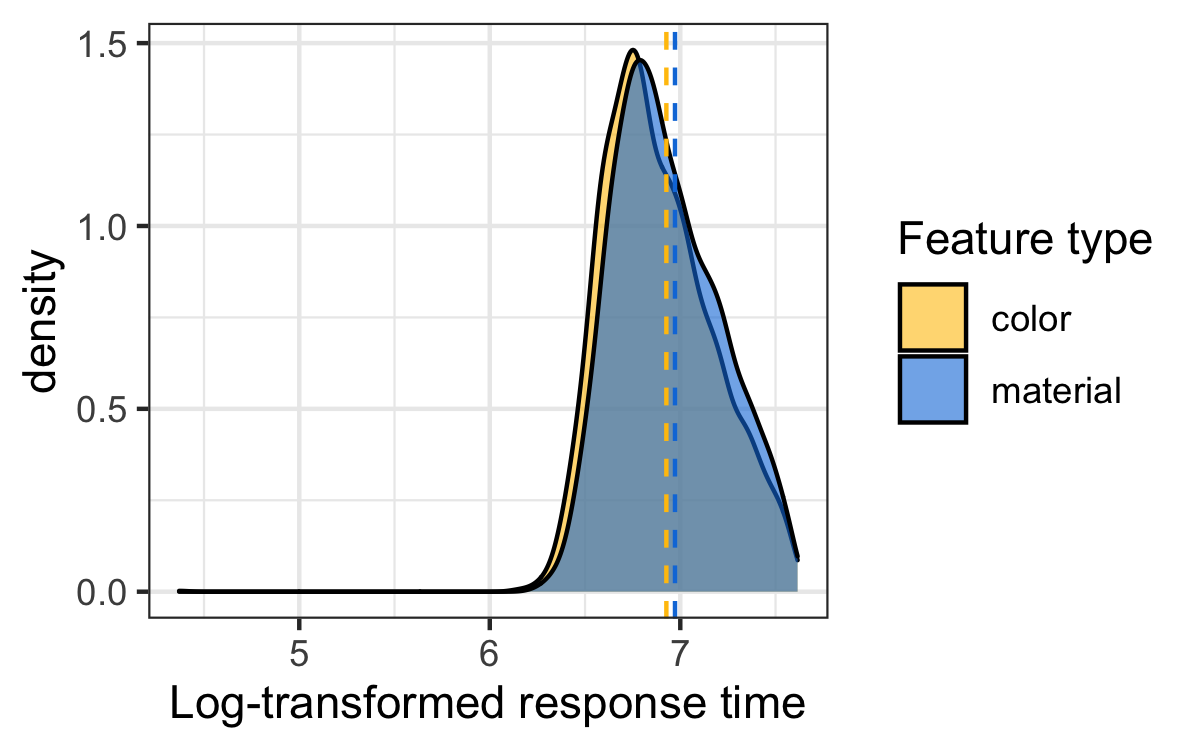
\includegraphics[width=\textwidth]{plots/exp1_density_logRT.png}
%    \caption{Exp.~1}
%    \label{fig:density_1}
%    \end{subfigure} \hspace{9mm}
%    \begin{subfigure}{.3\textwidth}
%    \centering
%    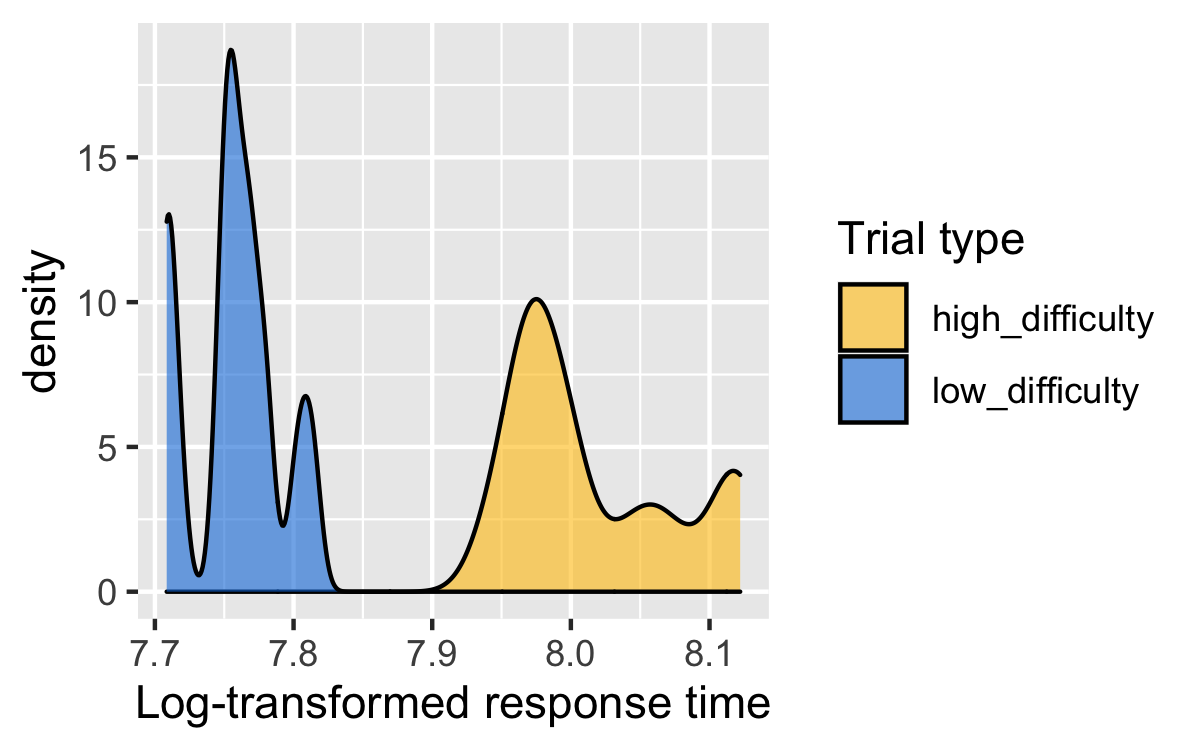
\includegraphics[width=\textwidth]{plots/exp23_density_logRT.png}
%    \caption{Exp.~2}
%    \label{fig:density_2}
%    \end{subfigure}
%    \begin{subfigure}{.3\textwidth}
%    \centering
%    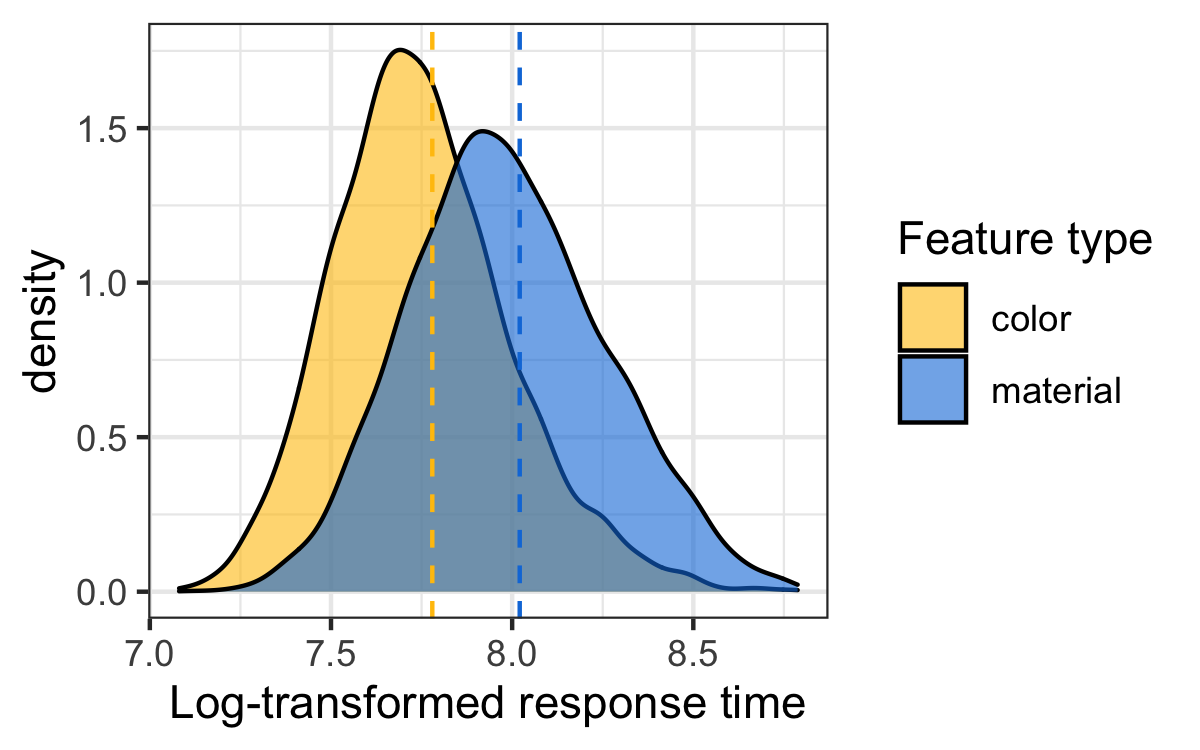
\includegraphics[width=\textwidth]{plots/exp3_density_logRT.png}
%    \caption{Exp.~3}
%    \label{fig:density_3}
%    \end{subfigure}
%    \caption{Distribution of log-transformed response times to adjectives tested in different experiments}
%    \label{fig:density}
% \end{figure}  

% \section{Citations and references} Use author-date notation for in-text citations, for example: ... as noted recently by Jameson (2012) and Mateus (2014), drawing on insights from various other researchers (e.g., Nelson 1986:223–28, Martin 2003, Wellington \& Johnson 2016), there have been numerous technological advances in the procedures used to publish research articles online. Include URLs or DOIs with active hyperlinks in citations. The \textit{Semantics and Pragmatics} stylesheet \href{https://raw.githubusercontent.com/semprag/tex/master/sp.bst}{sp.bst} meets the LSA formatting requirements for the list of references, and so may be used. See \href{http://info.semprag.org}{info.semprag.org}. 
% ------------ references --------------------------------------------------------------------------------------
\setlength{\bibsep}{0pt plus 0.3ex}
\setlength{\bibhang}{0.3in}			% hanging indent for references must be 0.3in
\titleformat{\section}{\normalfont\bfseries}{\thesection}{.5em}{}		
% references section not supposed to be followed by a period

\bibliographystyle{sp.bst}	
% \bibliographystyle{apacite}

% S\&P bibliography style
% S\&P, an LSA publication, meets the LSA guidelines. 
% See: http://info.semprag.org 
% and get the bst at: https://raw.githubusercontent.com/semprag/tex/master/sp.bst 
% If using the sp.bst, the following command turns your DOIs into links
\newcommand{\doi}[1]{\href{http://dx.doi.org/#1}{http://dx.doi.org/#1}}	%modified from sp.cls

\bibliography{pd-references}			% your bib file

\end{document}